% Copyright 2026 Sreeram Anil
% SPDX-License-Identifier: CC-BY-4.0
% =============================================================================
%  Square-root extended Kalman filter (QR array algorithm) — classical Kalman family
% =============================================================================
\chapter{Square-Root Extended Kalman Filter (SR-EKF)}
\label{ch:srekf}

\section*{At a glance}
\begin{tabular}{@{}l>{\raggedright\arraybackslash}p{0.76\textwidth}@{}}
Family & classical Kalman (factored) \\
Header & \texttt{include/estkit/filters/srekf.hpp} \\
Registered name & \texttt{SR-EKF} \\
State dimension & $n_x = 4$ (cell model) --- generic in $n_x, n_u, n_y$ \\
Propagated quantity & $\mS$ with $\mP = \mS\mS^\T$ (lower triangular) \\
Cost per step & $\mathcal{O}(n_x^3)$ (two Householder QRs); $0.78$--$0.83\,\SI{}{\micro\second}$/step \\
Primary references & \cite{kaminski1971,kailath2000,potter1963,carlson1973,verhaegen1986} \\
\end{tabular}

\section{Motivation and aerospace/BMS relevance}
Square-root filtering was invented for flight. Potter's scalar square-root update was written
for the Apollo on-board navigation filter~\cite{potter1963} because the guidance computer's
short word length made the conventional covariance recursion lose positive definiteness;
Andrews~\cite{andrews1968sqrt}, Carlson~\cite{carlson1973} and the survey of Kaminski, Bryson
and Schmidt~\cite{kaminski1971} turned it into the standard formulation for orbit
determination and inertial navigation, and Verhaegen and Van Dooren's error
analysis~\cite{verhaegen1986} established the modern statement: a square-root
implementation has the numerical behaviour of a conventional one run with twice the mantissa
length.

The relevance to battery management is direct. A BMS runs on a microcontroller, often in
single precision, often for thousands of hours without a reset, and it must never produce a
non-physical covariance --- a negative variance on SOC would propagate into the reserve
computation. A square-root filter makes $\mP\succeq0$ a structural property rather than a
numerical hope, at a cost of roughly $50\,\%$ more arithmetic, and it does so without
changing a single estimate.

\section{Problem statement and assumptions}
Model \eqref{eq:ekf-proc}--\eqref{eq:ekf-meas}, differentiable $f$ and $h$ (this is an EKF:
Jacobians are used). Factors $\mS_Q$, $\mS_R$ with $\mQ=\mS_Q\mS_Q^\T$, $\mR=\mS_R\mS_R^\T$
are computed per step by \code{cholesky\_safe}. The filter propagates $\mS$ with
$\mP=\mS\mS^\T$, $\mS$ lower triangular with non-negative diagonal, which makes the factor
unique.

\section{Derivation}
The operator $\operatorname{Tria}$ of \eqref{eq:sckf-tria} --- the lower-triangular factor of
$\mA\mA^\T$ obtained from the QR of $\mA^\T$ --- is the only tool required.

\paragraph{Time update.} $\Pminus_k = \mF\Pplus_{k-1}\mF^\T + \mQ$ is a sum of two
Gram matrices,
\begin{equation}
\Pminus_k = (\mF\mS^+_{k-1})(\mF\mS^+_{k-1})^\T + \mS_Q\mS_Q^\T
 = \left[\mF\mS^+_{k-1}\;\;\mS_Q\right]\left[\cdot\right]^\T
 \;\Longrightarrow\;
 \mS^-_k = \operatorname{Tria}\!\left(\left[\mF\mS^+_{k-1}\;\;\mS_Q\right]\right),
\label{eq:srekf-tu}
\end{equation}
an $n_x\times 2n_x$ pre-array. No subtraction occurs, so $\Pminus_k$ is positive
semi-definite by construction.

\paragraph{Measurement update: the array algorithm.} The elegance of the square-root form is
that the gain, the innovation covariance factor and the posterior factor all fall out of
\emph{one} orthogonal triangularisation~\cite[Ch.~12]{kailath2000}. Consider the
$(n_y+n_x)\times(n_y+n_x)$ pre-array and its triangularisation
\begin{equation}
\mB = \begin{bmatrix} \mS_R & \mH\mS^-_k \\[2pt] \bm{0} & \mS^-_k \end{bmatrix},
\qquad
\mL = \operatorname{Tria}(\mB) = \begin{bmatrix} \mS_e & \bm{0} \\[2pt] \mK_p & \mS^+_k \end{bmatrix}.
\label{eq:srekf-array}
\end{equation}
Both sides have the same Gram matrix, and
\begin{equation}
\mB\mB^\T = \begin{bmatrix}
\mR + \mH\Pminus_k\mH^\T & \mH\Pminus_k \\
\Pminus_k\mH^\T & \Pminus_k \end{bmatrix},
\qquad
\mL\mL^\T = \begin{bmatrix}
\mS_e\mS_e^\T & \mS_e\mK_p^\T \\
\mK_p\mS_e^\T & \mK_p\mK_p^\T + \mS^+_k\mS^{+\T}_k \end{bmatrix}.
\label{eq:srekf-gram}
\end{equation}
Equating blocks gives, in order,
\begin{align}
\mS_e\mS_e^\T &= \mH\Pminus_k\mH^\T + \mR = \mS_k \quad \text{(innovation covariance)},
\label{eq:srekf-Se}\\
\mK_p &= \Pminus_k\mH^\T\mS_e^{-\T} \;\Longrightarrow\;
 \mK_k = \Pminus_k\mH^\T\mS_k\inv = \mK_p\mS_e\inv,
\label{eq:srekf-Kp}\\
\mS^+_k\mS^{+\T}_k &= \Pminus_k - \mK_p\mK_p^\T
 = \Pminus_k - \Pminus_k\mH^\T\mS_k\inv\mH\Pminus_k = \Pplus_k,
\label{eq:srekf-Sp}
\end{align}
i.e. exactly the Kalman gain and the Kalman covariance update, obtained without forming any
inverse and without any subtraction of matrices (the ``subtraction'' \eqref{eq:srekf-Sp} is
performed implicitly by the orthogonal rotations, which cannot produce an indefinite result).
The state update needs one forward substitution:
\begin{equation}
\xplus_k = \xminus_k + \mK_p\left(\mS_e\inv\bm{\veps}_k\right), \qquad
\bm\veps_k = \vy_k - h(\xminus_k,\vu_k).
\label{eq:srekf-state}
\end{equation}

\paragraph{Potter's form.} For a scalar measurement ($n_y=1$) the original
formulation~\cite{potter1963} avoids the QR entirely. With $\mP = \mS\mS^\T$, $\mS$ a
\emph{symmetric} (not triangular) square root, and $\bm\phi = \mS^\T\mH^\T$,
\begin{equation}
a = \frac{1}{\bm\phi^\T\bm\phi + R}, \qquad
\mK = a\,\mS\bm\phi, \qquad
\mS^+ = \mS\left(\mI - a\gamma\,\bm\phi\bm\phi^\T\right), \quad
\gamma = \frac{1}{1+\sqrt{aR}},
\label{eq:srekf-potter}
\end{equation}
a rank-one modification costing $\mathcal{O}(n_x^2)$ per scalar measurement --- cheaper than
the array form, which is why it was chosen for Apollo. Its limitations are that it handles
one measurement at a time, that it does not produce a triangular factor (so a separate
factorisation is needed for the time update), and that $\mQ$ must be handled separately.
Carlson~\cite{carlson1973} fixed the first two by deriving a triangular version. The array
form \eqref{eq:srekf-array} is preferred here because it handles vector measurements and
process noise uniformly and maps onto one library primitive.

\section{Algorithm}
\begin{algorithm}[H]
\caption{SR-EKF --- one sampling period}
\begin{algorithmic}[1]
\Require $\xplus_{k-1},\mS^+_{k-1},\vu_{k-1},\vy_k,\vu_k$
\State \textbf{Time update:} $\mF\gets\partial f/\partial\vx|_{\xplus_{k-1},\vu_{k-1}}$;\;
       $\xminus_k\gets f(\xplus_{k-1},\vu_{k-1})$
\State $\mS_Q\gets\operatorname{chol}(\mQ)$;\;
       $\mS^-_k\gets\operatorname{Tria}\!\left(\left[\mF\mS^+_{k-1}\;\;\mS_Q\right]\right)$
\State \textbf{Predicted measurement:} $\yhat_k\gets h(\xminus_k,\vu_k)$
\State \textbf{Measurement update:} $\mH\gets\partial h/\partial\vx|_{\xminus_k,\vu_k}$;\;
       $\mS_R\gets\operatorname{chol}(\mR)$
\State $\begin{bmatrix}\mS_e&\bm0\\ \mK_p&\mS^+_k\end{bmatrix}
        \gets \operatorname{Tria}\!\left(\begin{bmatrix}\mS_R&\mH\mS^-_k\\ \bm0&\mS^-_k\end{bmatrix}\right)$
\State $\bm w\gets\mS_e\inv(\vy_k-\yhat_k)$ \Comment{forward substitution}
\State $\xplus_k\gets\xminus_k+\mK_p\bm w$
\State \textbf{if} constraints enabled \textbf{then} $\xplus_k\gets\Pi(\xplus_k)$
\Ensure $\xplus_k,\mS^+_k$ \quad ($\mP$ reconstructed on demand as $\mS^+\mS^{+\T}$)
\end{algorithmic}
\end{algorithm}

\section{Application to the battery model}
For $n_x=4$, $n_y=1$ the pre-arrays are $4\times8$ (time update) and $5\times5$ (measurement
update). Because $\mF = \diag(1,a_1,a_2,a_h)$ the product $\mF\mS$ is a row scaling, so the
time-update pre-array costs $n_x^2$ multiplies plus the QR. The measurement pre-array is
square, so $\operatorname{Tria}$ is a $5\times5$ Householder QR --- $\approx 150$ flops. The
total, $0.78$--$0.83\,\SI{}{\micro\second}$ per step, is $\approx 70\,\%$ above the
conventional EKF's $0.44$--$0.48$, consistent with the standard estimate for array
algorithms.

The benchmark reports $\sigma_\soc$, so the filter must expose $\mP$; it does so through a
cached $\mS\mS^\T$ that is recomputed only when $\mS$ has changed and only if the accessor is
called. A production implementation would read $\sigma_\soc$ directly off the first row of
$\mS$ as $\sqrt{\sum_j S_{1j}^2}$ and never form $\mP$ at all.

\section{Implementation notes}
The whole filter is 40 lines on top of \code{qr\_r}. \code{cholesky\_safe} guarantees that
$\mS_Q$ and $\mS_R$ exist even for a numerically semi-definite $\mQ$; \code{qr\_r} forces a
non-negative diagonal so that the factor is unique and the recursion is bit-reproducible.
Guards: if $\mS_e\inv\bm\veps$ or the posterior factor is not finite, the update is skipped
and the prior is kept. \code{sizeof(SqrtEkf<EcmModel>)} is 4440\,bytes, $104$\,bytes more
than the EKF (the cached $\mP$).

\paragraph{When the factorisation actually pays.} The peak condition number of $\mP$ along
the eVTOL mission is $\kappa\approx1.3\times10^6$ (final value $6.9\times10^3$). In single
precision $\kappa\varepsilon\approx0.16$ for the covariance form --- uncomfortably close to
losing all significance in the smallest eigenvalue --- against
$\sqrt{\kappa}\,\varepsilon\approx1.4\times10^{-4}$ for the square-root form. That the
conventional EKF nevertheless survives here is a consequence of the Joseph form and of the
process-noise floor $q_{\text{floor}}$, which keeps the smallest eigenvalue away from zero.
Remove either safeguard, add near-deterministic states (parameter augmentation with
$q_\theta\to0$) or move to fixed point, and the covariance form fails while
\eqref{eq:srekf-array} does not.

\section{Benchmark results}
% Copyright 2026 Sreeram Anil
% SPDX-License-Identifier: CC-BY-4.0
\begin{table}[H]\centering\footnotesize\setlength{\tabcolsep}{4pt}
\caption{SR-EKF: cell-level benchmark on the eVTOL mission (mean over seeds; RMSE and max error in \% SOC; $t_\mathrm{conv}$: first time the error stays below 2\,\% for 60\,s, -- = never; EKF reference: steady-state RMSE of the plain EKF on the same data).}\label{tab:cell_SREKF}
\begin{tabular}{llrrrrrcrr}\toprule
plant & scenario & RMSE & RMSE$_\mathrm{ss}$ & max & $t_\mathrm{conv}$ [s] & RMSE$_v$ [mV] & div. & EKF ref. & ns/step \\ \midrule
ECM & nominal & 0.15 & 0.05 & 1.07 & 0 & 0.79 & no & 0.05 & 821 \\
ECM & init\_error & 0.14 & 0.05 & 0.62 & 0 & 2.12 & no & 0.05 & 823 \\
ECM & current\_bias & 0.54 & 0.61 & 1.40 & 0 & 0.86 & no & 0.61 & 825 \\
ECM & noise\_step & 0.18 & 0.12 & 1.07 & 0 & 2.89 & no & 0.12 & 826 \\
ECM & outliers & 0.52 & 0.21 & 2.92 & 16 & 2.05 & no & 0.21 & 829 \\
ECM & cold & 0.20 & 0.16 & 1.17 & 0 & 1.90 & no & 0.16 & 823 \\
ECM & hot & 0.20 & 0.03 & 1.01 & 0 & 0.54 & no & 0.03 & 822 \\
ECM & aged\_cell & 1.18 & 1.52 & 2.96 & 0 & 3.80 & no & 1.52 & 827 \\
ECM & param\_mismatch & 1.28 & 1.36 & 2.87 & 0 & 2.80 & no & 1.36 & 829 \\
ECM & sensor\_dropout & 0.72 & 0.46 & 2.27 & 0 & 1.73 & no & 0.46 & 827 \\
ECM & preisach & 0.58 & 0.20 & 1.67 & 16 & 0.81 & no & 0.20 & 824 \\
ECM & combined & 16.02 & 12.44 & 29.64 & -- & 5.15 & no & 12.44 & 822 \\
\midrule
SPM & nominal & 3.65 & 3.73 & 4.31 & 0 & 1.02 & no & 3.73 & 790 \\
SPM & init\_error & 3.78 & 3.81 & 4.59 & 0 & 2.18 & no & 3.81 & 787 \\
SPM & current\_bias & 4.93 & 5.69 & 6.39 & 0 & 1.12 & no & 5.69 & 789 \\
SPM & noise\_step & 3.42 & 3.30 & 4.31 & 0 & 3.14 & no & 3.30 & 788 \\
SPM & outliers & 2.07 & 1.99 & 3.44 & 3 & 2.27 & no & 1.99 & 794 \\
SPM & cold & 7.07 & 7.35 & 9.65 & 0 & 4.49 & no & 7.35 & 784 \\
SPM & hot & 2.08 & 2.16 & 2.42 & 0 & 0.69 & no & 2.16 & 792 \\
SPM & param\_mismatch & 2.87 & 3.13 & 3.61 & 0 & 1.96 & no & 3.13 & 788 \\
SPM & sensor\_dropout & 5.13 & 5.31 & 5.96 & 0 & 1.95 & no & 5.31 & 789 \\
\bottomrule\end{tabular}\end{table}

\begin{figure}[H]\centering
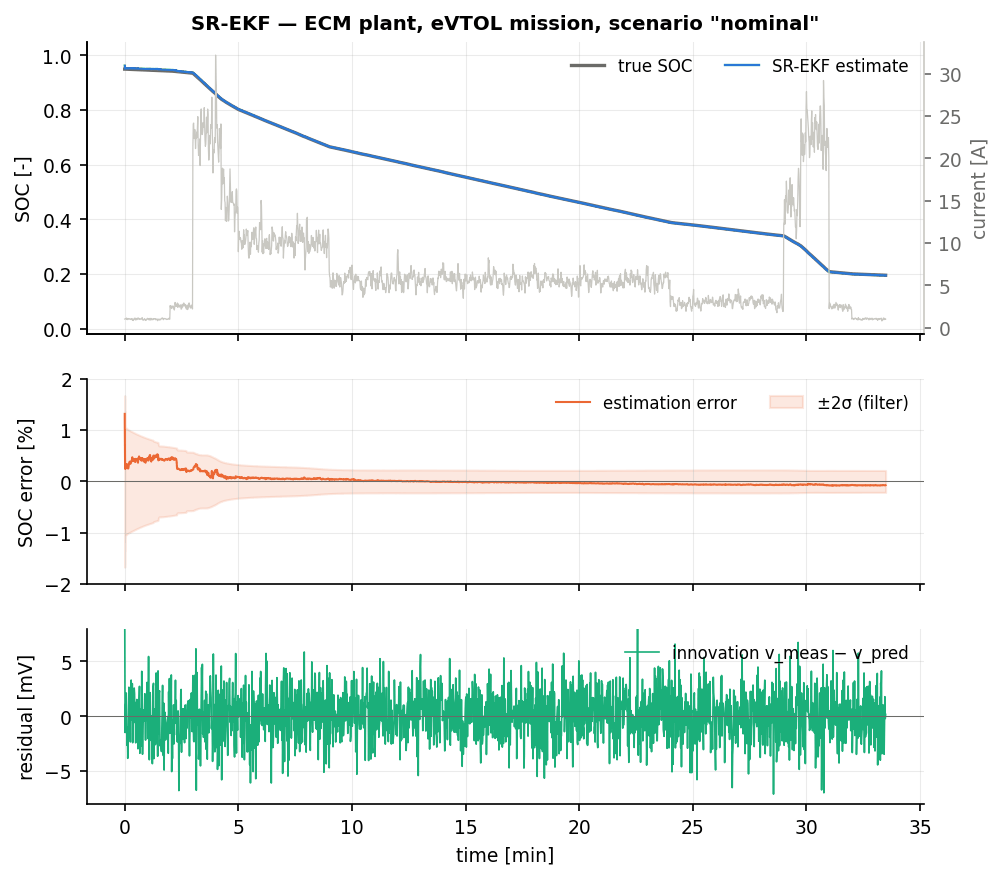
\includegraphics[width=\textwidth]{figures/cell_SREKF_nominal.png}
\caption{SR-EKF on the nominal eVTOL mission: true and estimated SOC (top), estimation error with the $\pm 2\sigma$ band when available (middle), voltage residual (bottom).}
\end{figure}
\begin{figure}[H]\centering
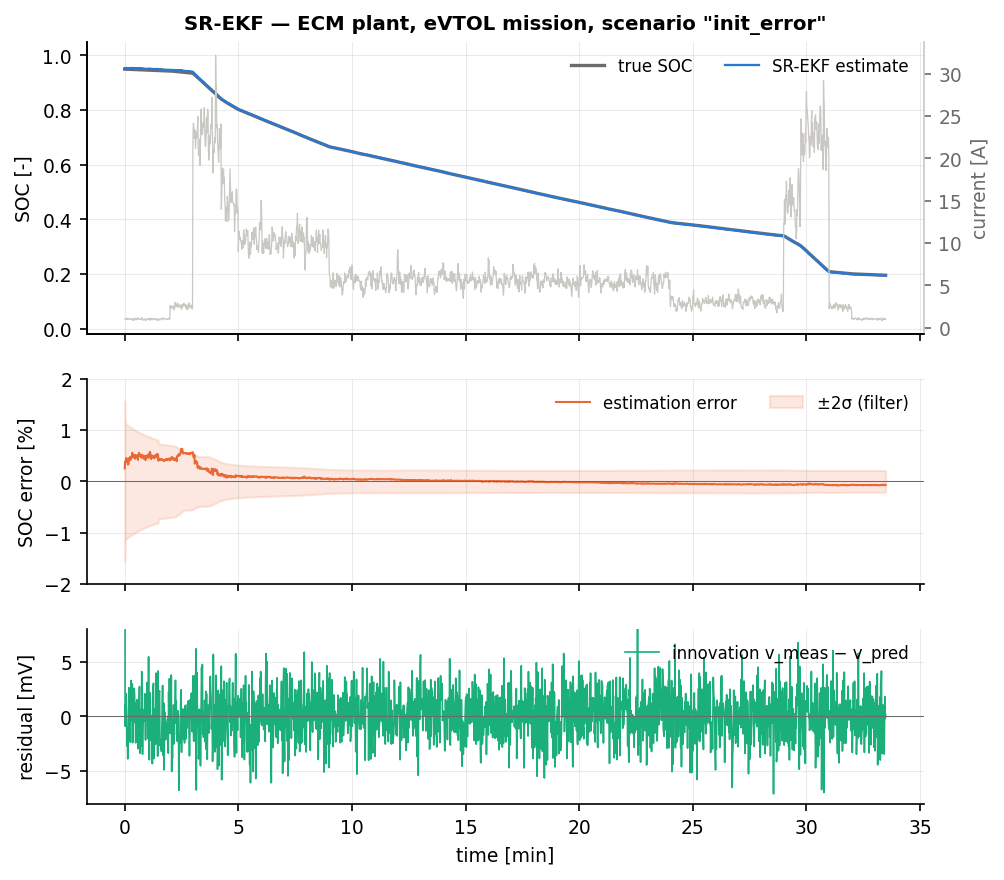
\includegraphics[width=\textwidth]{figures/cell_SREKF_init_error.png}
\caption{SR-EKF with a 35\,\% initial SOC error.}
\end{figure}

All numbers are three-seed means in per cent SOC.

The SR-EKF matches the EKF on all twelve ECM scenarios to two decimals: \texttt{nominal}
$0.15/0.05\,\%$, \texttt{init\_error} $0.14/0.05\,\%$ with $t_{\text{conv}} = 0$\,s,
\texttt{current\_bias} $0.54/0.61\,\%$, \texttt{cold} $0.20/0.16\,\%$, \texttt{aged\_cell}
$1.18/1.52\,\%$, \texttt{param\_mismatch} $1.28/1.36\,\%$, \texttt{sensor\_dropout}
$0.72/0.46\,\%$, \texttt{preisach} $0.58/0.20\,\%$, \texttt{combined} $16.02/12.44\,\%$ (never
converges). A direct element-wise comparison over a full mission gives
$\max\abs{\Delta\vx} = 3.1\times10^{-14}$ and $\max\abs{\Delta\mP} = 4.0\times10^{-15}$ --- the
tightest agreement of the three EKF-equivalent implementations (the U-D filter is at
$1.6\times10^{-14}$, the information filter at $1.9\times10^{-11}$), which is itself a small
piece of evidence for the conditioning argument above. All estimation-behaviour discussion in
Chapter~\ref{ch:ekf} applies verbatim, including the \texttt{combined} failure, which is an
approximation failure and not a numerical one.

In the single-precision build the nominal steady-state RMSE is $0.06\,\%$ for both forms, and
on \texttt{aged\_cell} the square-root form is marginally better ($1.47\,\%$ against the
conventional EKF's $1.48\,\%$, both against $1.39\,\%$ in double); on \texttt{combined} both
give $12.2\,\%$. The cell problem at $n_x = 4$ simply is not ill-conditioned enough for the two
to separate. A deliberate stress test in float (scaling $\mR$ down by $10^4$, i.e. pretending
the voltage sensor is $100\times$ more accurate than it is, which drives $\kappa(\mP)$ up) gave
$\text{RMSE}_{\text{ss}} = 0.79\,\%$ for the SR-EKF against $2.39\,\%$ for the EKF; but that
experiment changes the estimator's statistics as well as its conditioning --- the U-D filter of
Chapter~\ref{ch:udekf}, which is equally well conditioned, came out at $5.07\,\%$ --- so it is
reported as an indication only and not as a controlled demonstration.

The runtime penalty, $\approx 70\,\%$ ($0.78$--$0.83\,\SI{}{\micro\second}$ against the EKF's
$0.44$--$0.48$), is the honest cost. Against it: a covariance that cannot go indefinite, a
branch-free deterministic instruction count, and no matrix inverse anywhere in the cycle.

\paragraph{SPM plant: structured model error.}
\begin{figure}[H]\centering
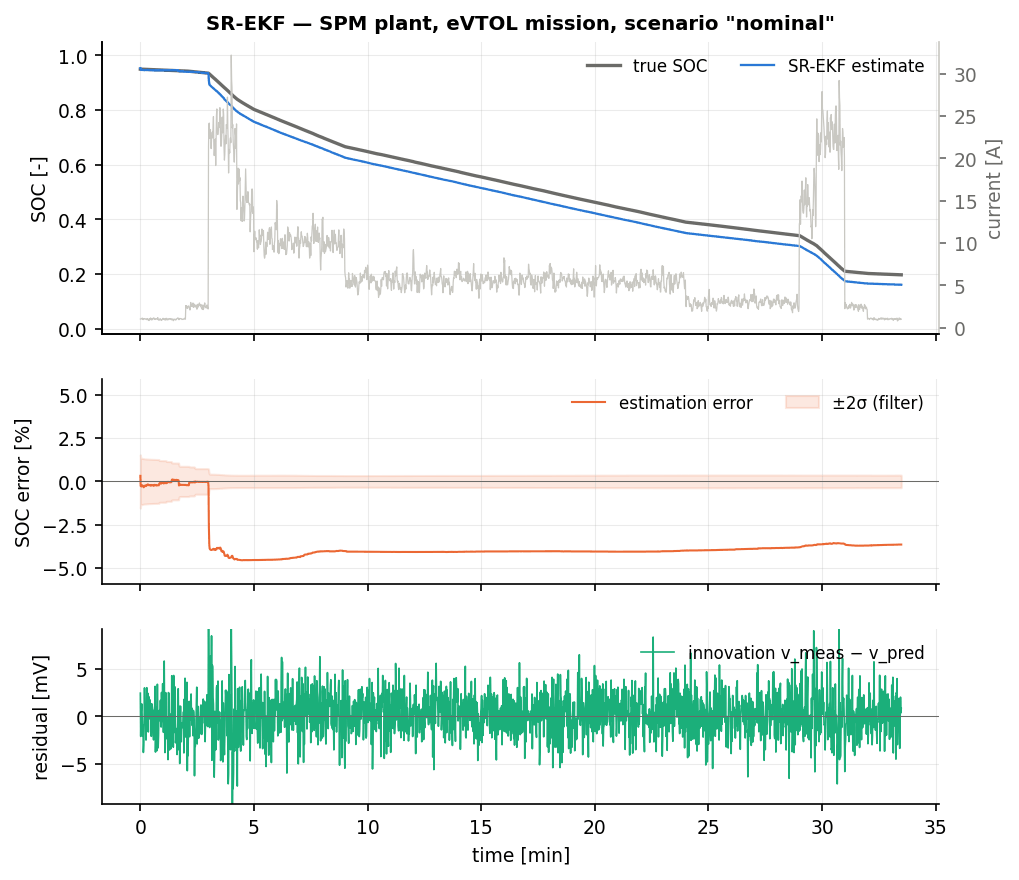
\includegraphics[width=\textwidth]{figures/cellspm_SREKF_nominal.png}
\caption{SR-EKF on the nominal mission with the electrochemical (SPM) plant; identical to the conventional EKF.}
\end{figure}
The SPM block of the table is a different kind of test. The plant is the electrochemical
single-particle model; the estimator still runs a 2-RC equivalent circuit, fitted to that plant,
which leaves a \emph{structured} residual of about $4$\,mV (Butler--Volmer kinetics and
solid-phase diffusion that no 2-RC circuit can reproduce) and a slow second branch,
$\tau_2 = 556$\,s. Over a $33$-minute mission a $556$\,s pole barely relaxes, so $v_2(t)$ is
close to an affine ramp --- and so is $\ocv(\soc(t))$ while the cell discharges at a roughly
constant rate. The two channels through which the measurement sees the state,
$(\partial\ocv/\partial\soc)\,\delta\soc$ and $-\delta v_2$, are therefore nearly collinear in
the information accumulated over the flight: the pair $(\soc, v_2)$ is close to unobservable,
and no filter can decide whether a persistent few-millivolt residual belongs to the slow RC
branch or to the state of charge. Because that direction is weakly observable, a $4$\,mV
structured error maps onto \emph{several per cent} of SOC instead of the
$4\,\text{mV}/0.8\,\text{V}\approx0.5\,\%$ a well-conditioned channel would give. This
$(\soc,v_2)$ ambiguity, not the size of the residual, is the mechanism behind the
$3.7$--$4.6\,\%$ band in which the whole classical family sits.

Being algebraically the EKF, this filter inherits the EKF's SPM rows exactly:
$3.65/3.73\,\%$ on \texttt{nominal} with a voltage residual of only $1.02$\,mV,
$7.35\,\%$ on \texttt{cold}, $5.69\,\%$ on \texttt{current\_bias}, $5.31\,\%$ on
\texttt{sensor\_dropout}, $3.13\,\%$ on \texttt{param\_mismatch} and $1.99\,\%$ on
\texttt{outliers}. Fitting the voltage to a millivolt while being $4\,\%$ wrong about SOC is
the signature of the ambiguity: the filter pays for the fit with $v_2$ and $\soc$ in the wrong
proportion. Nothing diverges and $t_{\text{conv}} = 0$ on every SPM row --- the error is a
bias, not a drift. Within the family the tangent-linearising filters (EKF, IEKF and these three
re-implementations) are at the \emph{good} end of the band, because a tangent commits less
weight to the badly conditioned OCV channel than a wide statistical regression does; only the
frozen-linearisation LKF ($1.72\,\%$, Chapter~\ref{ch:lkf}) and the second-order EKF
($3.52\,\%$) do better.

\section{Summary}
The array square-root EKF is the EKF with the numerics fixed: identical estimates to
$10^{-14}$, a structurally positive semi-definite covariance, no inverses, and one clean
primitive (\code{Tria}) doing all the work. Use it whenever the target is single precision or
fixed point, whenever the state contains near-deterministic components (augmented parameters,
biases), or whenever certification requires that a negative variance be impossible by
construction rather than by argument. On a double-precision desktop run of this benchmark it
buys nothing but costs $70\,\%$ --- which is the correct way to read every square-root result
in this report. Note that the U-D form of Chapter~\ref{ch:udekf} obtains the same guarantee for
no extra cost at all when $n_y = 1$.
